\documentclass[11pt]{article}
\usepackage{amsmath,amssymb,booktabs,graphicx}
\usepackage[margin=1in]{geometry}

\title{MVP Simulator: MDP Formulation, Contextual Bandits, and Benchmark Results}
\author{William Dennis}
\date{June 2026}

\begin{document}
\maketitle

\section{MDP Formulation}

The MVP simulator implements a finite-horizon MDP $(\mathcal{S}, \mathcal{A}, P, r, \gamma, T)$:

\subsection{State Space}
\[
\mathcal{S} = \{\texttt{sedentary},\ \texttt{active}\}
\]
Two activity states with no additional time-of-day dimension. Time-dependent reward scaling is handled via \texttt{reward\_multiplier\_by\_step} (see \S\ref{sec:reward} below).

\subsection{Action Space}
\[
\mathcal{A} = \{\texttt{nudge},\ \texttt{idle}\}
\]
A binary intervention: send a motivational message (\texttt{nudge}) or do not (\texttt{idle}).

\subsection{Transition Function}

$P(s' \mid s, a)$ is a configurable $2 \times 2 \times 2$ tensor. Rows index current state $s \in \{\text{sedentary}, \text{active}\}$ and columns index next state $s'$ in the same order:

\[
P_{\text{nudge}} =
\begin{bmatrix}
0.7 & 0.3 \\[2pt]
0.5 & 0.5
\end{bmatrix}
\qquad
P_{\text{idle}} =
\begin{bmatrix}
0.9 & 0.1 \\[2pt]
0.4 & 0.6
\end{bmatrix}
\]

Sending a reminder increases $P(\text{active} \mid \text{sedentary})$ from $0.1$ to $0.3$ but decreases $P(\text{active} \mid \text{active})$ from $0.6$ to $0.5$, consistent with Reactance theory (reminders can backfire for already-active users).

Optional \texttt{reward\_multiplier\_by\_step}: a per-step scaling factor that can zero out rewards at certain daily steps (soft mask). When absent, all multipliers default to 1.0. The per-step reward is computed as $\text{base reward} \times \text{multiplier}[t]$ where $t$ is the step-of-day index.

\subsection{Reward}\label{sec:reward}

The base reward is a vector indexed by next state:

\[
r = [0.0,\; 1.0]^\top \quad (\text{sedentary},\; \text{active})
\]

The per-step reward at time $t$ scales by the multiplier:

\[
r(s, a, t) = m[t \bmod S] \cdot r(s')
\]

where $S = \texttt{steps\_per\_day}$, $m \in \mathbb{R}^S$ is \texttt{reward\_multiplier\_by\_step}
(default $m_i = 1.0$), and $s'$ is the next state after taking action $a$ in state $s$.
Currently $m_i = 1.0$ for all $i$, so $r(s, a, t) = r(s')$.

Single-timescale placeholder. Multi-timescale reward (immediate + delayed body measure) is deferred to Phase 2.

\subsection{Episode Structure}
$T = \texttt{episode\_days} \times \texttt{steps\_per\_day}$ timesteps. Default: $T = 90 \text{ days} \times 5 \text{ steps/day} = 450$.

\section{Baseline Agents}

All agents in this section are state-blind bandits: they do not condition on the current activity state. From the transition matrix,
$E[r \mid \text{nudge}] \approx 0.375$, $E[r \mid \text{idle}] = 0.20$, and a
state-aware policy that nudges only when sedentary would achieve $\approx 0.429$.
This gap motivates the contextual agents in \S\ref{sec:contextual}.

\subsection{Thompson Sampling}
Beta-Bernoulli TS with prior $\text{Beta}(1, 1)$ per action. Posterior update:
\[
\alpha_a \leftarrow \alpha_a + \mathbb{1}[s'.\texttt{activity} = \texttt{active}], \quad
\beta_a \leftarrow \beta_a + \mathbb{1}[s'.\texttt{activity} = \texttt{sedentary}]
\]
Action selected by sampling $\theta_a \sim \text{Beta}(\alpha_a, \beta_a)$ and choosing $a^* = \arg\max_a \theta_a$.

\subsection{Epsilon-Greedy}
$\epsilon = 0.1$. With probability $\epsilon$, select uniformly at random; otherwise select $\arg\max_a Q(a)$. Q-values updated via incremental average:
\[
Q(a) \leftarrow Q(a) + \frac{r_t - Q(a)}{n_a}
\]

\subsection{UCB1}
Upper Confidence Bound with exploration parameter $c = 2.0$. Selects:
\[
a^* = \arg\max_a \left[ Q(a) + c \sqrt{\frac{\ln N}{N_a}} \right]
\]
where $N$ is total steps and $N_a$ is the number of times action $a$ was chosen. The confidence bonus shrinks as $N_a$ grows, naturally shifting from exploration to exploitation. Each action is pulled once before UCB is applied.

\subsection{Random Baseline}
Uniform random action selection. No learning. Serves as lower bound.
The mixture chain $P_{\text{random}} = \tfrac{1}{2}(P_{\text{nudge}} + P_{\text{idle}})$ gives $E[r] \approx 0.308$ per step, matching the empirical result within one standard deviation.

\section{Initial Results}

All agents run over 50 random seeds, 450 timesteps each. Results are reported as mean $\pm$ standard deviation across seeds.

\subsection{Standard Config (\texttt{configs/mvp.yaml})}
Four baseline agents (TS, EG, UCB, Random). Agent definitions and hyperparameters live in \texttt{docs/mvp/configs/mvp.yaml}.

\begin{table}[h]
\centering
\begin{tabular}{lrrr}
\toprule
Agent & Total Reward & Per Step & Last 50 Steps \\
\midrule
Thompson Sampling ($\alpha_0=\beta_0=1$) & 159.6 $\pm$ 12.7 & 0.355 & 0.373 \\
Epsilon-Greedy ($\epsilon=0.1$) & 158.1 $\pm$ 17.8 & 0.351 & 0.370 \\
UCB ($c=2.0$) & 148.4 $\pm$ 12.6 & 0.330 & 0.354 \\
Random & 137.3 $\pm$ 12.3 & 0.305 & 0.319 \\
\bottomrule
\end{tabular}
\caption{Results on \texttt{configs/mvp.yaml} (50 seeds, 450 timesteps). TS and $\epsilon$-greedy perform similarly; TS has lower variance. UCB ($c=2.0$) underperforms relative to the tuned value ($c=0.5$, see \S\ref{sec:benchmark}).}
\end{table}

\subsection{Masked Config (\texttt{docs/mvp/configs/mvp\_masked.yaml})}
\texttt{reward\_multiplier\_by\_step: [1, 1, 1, 1, 0]} -- step 4 (end of day) yields zero reward regardless of outcome. Results are 10 seeds.

\begin{table}[h]
\centering
\begin{tabular}{lrr}
\toprule
Agent & Total Reward & Mean Reward/Step \\
\midrule
Thompson Sampling ($\alpha_0=\beta_0=1$) & 126.6 $\pm$ 6.8 & 0.281 $\pm$ 0.015 \\
Epsilon-Greedy ($\epsilon=0.1$) & 127.3 $\pm$ 10.2 & 0.283 $\pm$ 0.023 \\
UCB ($c=2.0$) & 116.9 $\pm$ 8.6 & 0.260 $\pm$ 0.019 \\
Random & 107.8 $\pm$ 6.7 & 0.240 $\pm$ 0.015 \\
\bottomrule
\end{tabular}
\caption{Results on \texttt{docs/mvp/configs/mvp\_masked.yaml} (10 seeds, 450 timesteps). Reward drops $\approx 20\%$ across all agents, matching the $1/5$ masked fraction. Relative ordering is preserved.}
\end{table}

\section{Contextual Bandits}\label{sec:contextual}

Context $c_t = s_t.\texttt{activity} \in \{\texttt{sedentary}, \texttt{active}\}$. Each algorithm maintains separate parameters per $(c, a)$ pair:

\begin{itemize}
  \item \textbf{Thompson Sampling:} $(\alpha_{c,a}, \beta_{c,a})$ posteriors. Sample $\theta_{c_t, a} \sim \text{Beta}(\alpha_{c_t, a}, \beta_{c_t, a})$, pick $a^* = \arg\max_a \theta_{c_t, a}$.
  \item \textbf{Epsilon-Greedy:} $Q_{c,a}$ values. With probability $\epsilon$ explore, otherwise $a^* = \arg\max_a Q_{c_t, a}$.
  \item \textbf{UCB:} $a^* = \arg\max_a \left[ Q_{c_t, a} + c \sqrt{\ln(N_{c_t}) / n_{c_t, a}} \right]$ where $N_{c_t} = \sum_a n_{c_t, a}$.
  \item \textbf{Decaying Epsilon-Greedy:} Linear decay: $\epsilon_t = \max(\epsilon_{\min},\; \epsilon_{\text{start}} (1 - t / T_{\text{decay}}))$.
\end{itemize}

\subsection{Optimal Policy}
Nudge when sedentary ($0.3 > 0.1$), idle when active ($0.6 > 0.5$). Contextual bound: $E[r] = 3/7 \approx 0.429$ per step, $192.9$ total ($14.3\%$ above non-contextual optimal).

\section{Hyperparameter Optimisation}
Grid search over key parameters (50 seeds, 450 timesteps, both standard and contextual variants):
\[
\begin{aligned}
\text{EG:} &\quad \epsilon \in [0.01, 0.50], \; \Delta 0.05 \\
\text{D-EG:} &\quad \epsilon_{\text{start}} \in [0.1, 1.0], \; \Delta 0.1; \quad T_{\text{decay}} \in [25, 700], \; \Delta 25 \\
\text{UCB:} &\quad c \in [0.1, 10.0], \; \Delta 0.5
\end{aligned}
\]

\begin{figure}[h]
\centering
\begin{minipage}{0.32\textwidth}
  \centering
  
\includegraphics[width=\textwidth]{images/hyperparam_eg.pdf}
  \caption*{\small EG: $\epsilon$ vs reward}
  \label{fig:hyperparam-eg}
\end{minipage}\hfill
\begin{minipage}{0.32\textwidth}
  \centering
  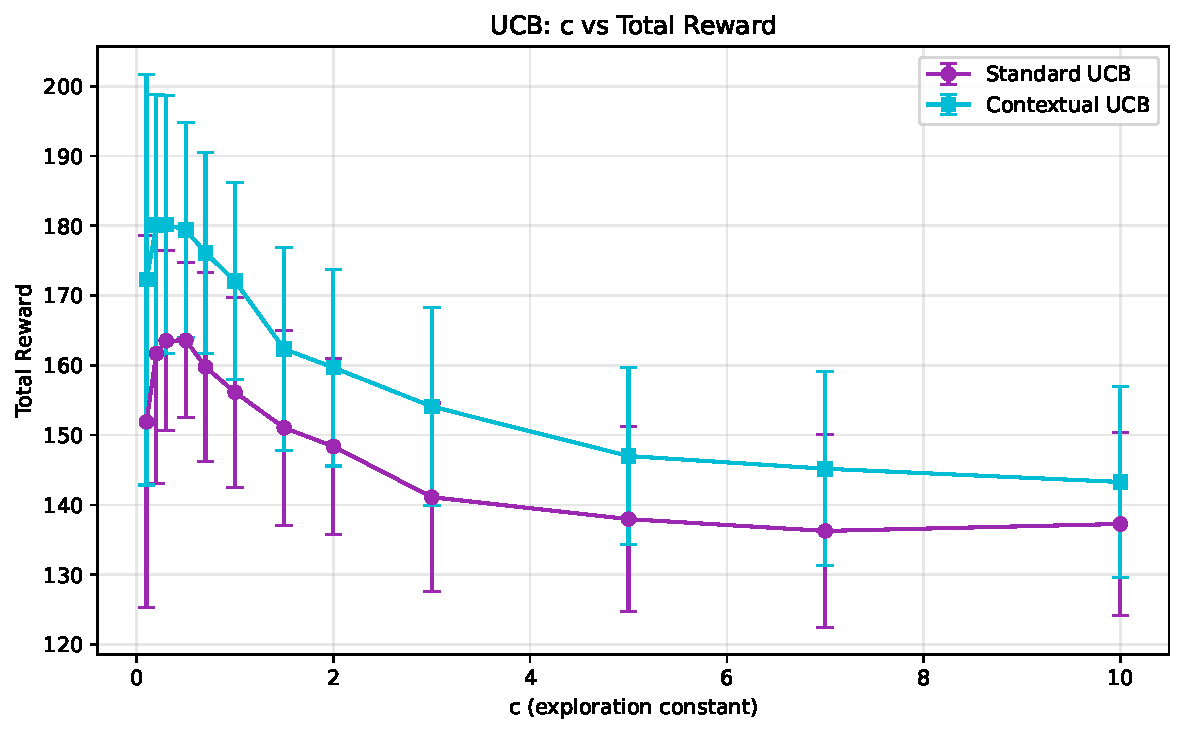
\includegraphics[width=\textwidth]{images/hyperparam_ucb.pdf}
  \caption*{\small UCB: $c$ vs reward}
  \label{fig:hyperparam-ucb}
\end{minipage}\hfill
\begin{minipage}{0.32\textwidth}
  \centering
  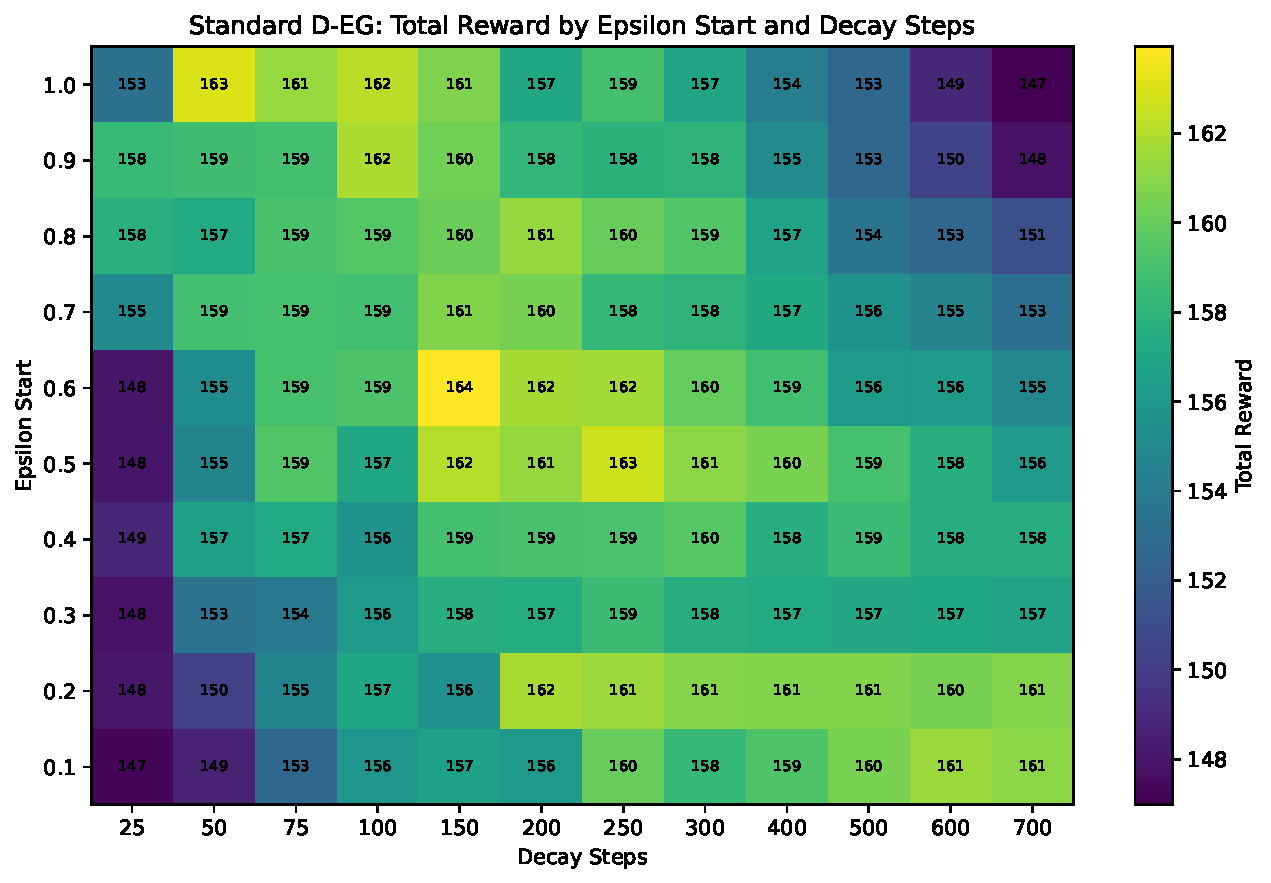
\includegraphics[width=\textwidth]{images/hyperparam_dec_heatmap.pdf}
  \caption*{\small D-EG: heatmap}
  \label{fig:hyperparam-dec-heatmap}
\end{minipage}
\caption{Hyperparameter sensitivity (50 seeds, $\pm$1~SD). EG optimum $\epsilon=0.15$, UCB optimum $c=0.5$ (both interior). D-EG total reward plateaus above $\epsilon_{\text{start}}=0.2$; $\epsilon_{\text{start}}=1.0$ is the theoretical maximum but $\epsilon_{\text{start}}=0.2$ is chosen in benchmarks for lower variance.}
\label{fig:hyperparam-all}
\end{figure}

$\epsilon=0.05$ vs $\epsilon=0.10$: identical means (158.1), but $\epsilon=0.10$ has $11\%$ lower variance.

\begin{figure}[h]
\centering
\begin{minipage}{0.32\textwidth}
  \centering
  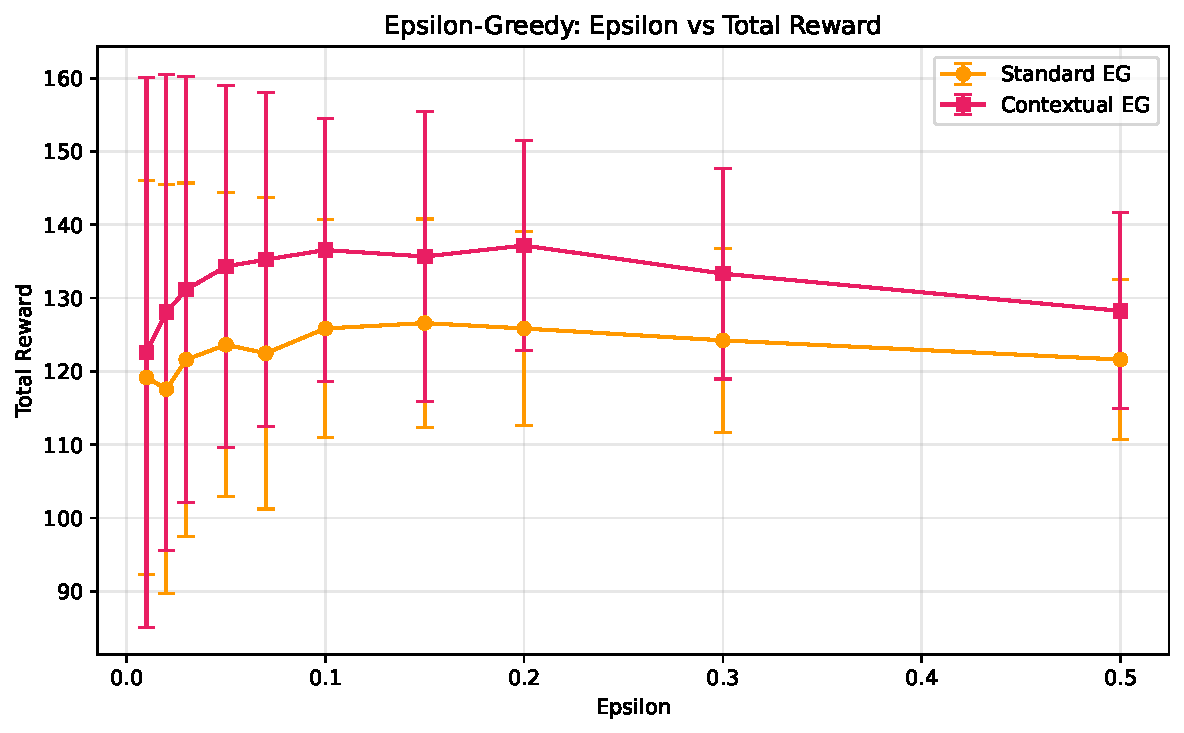
\includegraphics[width=\textwidth]{images/hyperparam_eg_masked.pdf}
  \caption*{\small EG (masked): $\epsilon$ vs reward}
  \label{fig:hyperparam-eg-masked}
\end{minipage}\hfill
\begin{minipage}{0.32\textwidth}
  \centering
  
\includegraphics[width=\textwidth]{images/hyperparam_ucb_masked.pdf}
  \caption*{\small UCB (masked): $c$ vs reward}
  \label{fig:hyperparam-ucb-masked}
\end{minipage}\hfill
\begin{minipage}{0.32\textwidth}
  \centering
  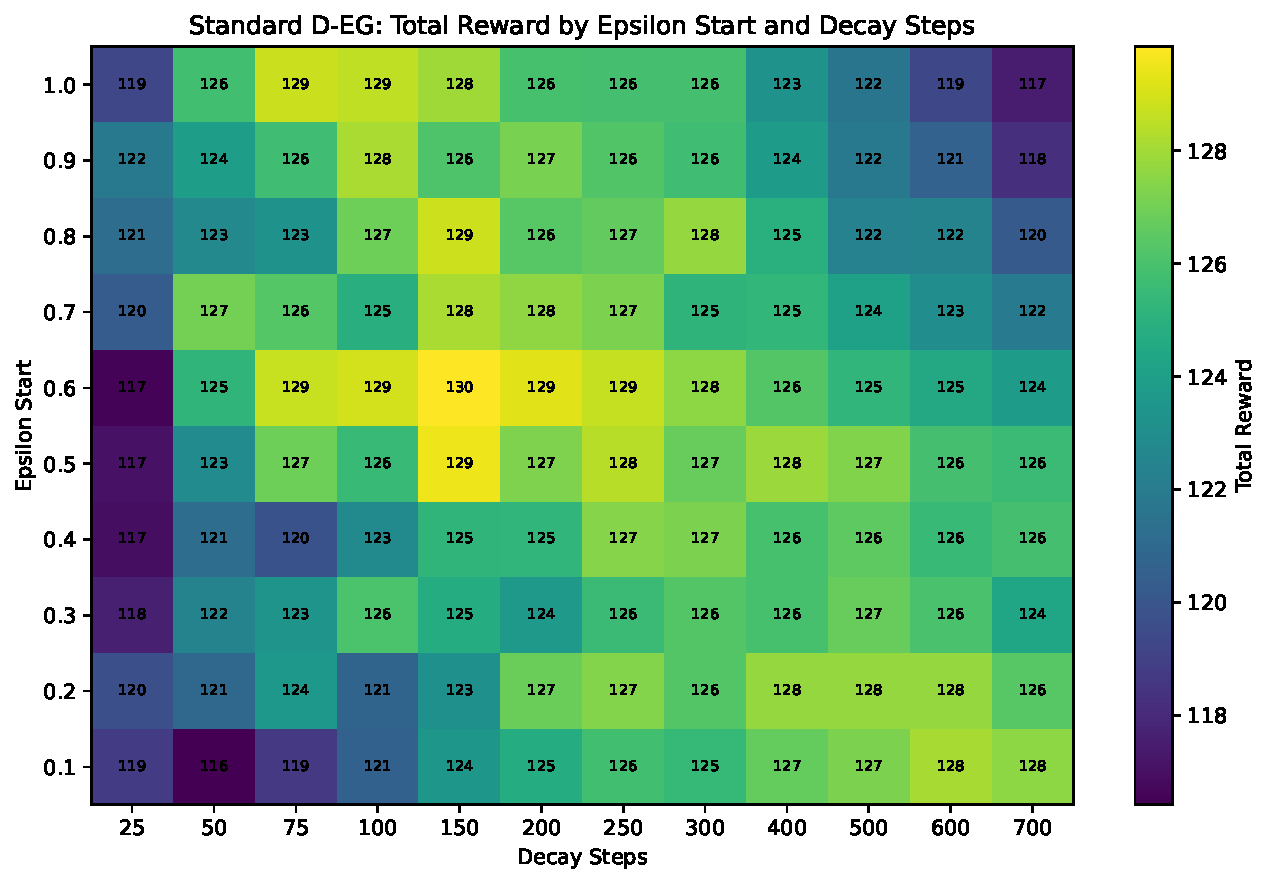
\includegraphics[width=\textwidth]{images/hyperparam_dec_heatmap_masked.pdf}
  \caption*{\small D-EG (masked): heatmap}
  \label{fig:hyperparam-dec-heatmap-masked}
\end{minipage}
\caption{Hyperparameter sensitivity under masked reward (50 seeds, $\pm$1~SD). Optima are unchanged from the non-masked case; the $20\%$ reward floor shift is uniform across all hyperparameter settings.}
\label{fig:hyperparam-masked-all}
\end{figure}

\section{Benchmark Results}\label{sec:benchmark}
50 seeds, 450 timesteps. Optimised hyperparameters: EG $\epsilon=0.05$, D-EG $\epsilon_{\text{start}}=0.2$, $T_{\text{decay}}=200$, $\epsilon_{\min}=0.01$, UCB $c=0.5$. All agent definitions live in \texttt{docs/mvp/configs/mvp\_extensions.yaml}.

\begin{table}[h]
\centering
\begin{tabular}{lrrrr}
\toprule
Agent & Total Reward & Per Step & Last 50 Steps & vs Contextual Opt \\
\midrule
Contextual UCB & 179.4 $\pm$ 15.4 & 0.399 & 0.430 & $-7.0\%$ \\
Contextual TS & 178.7 $\pm$ 15.8 & 0.397 & 0.429 & $-7.4\%$ \\
Contextual EG & 166.6 $\pm$ 30.4 & 0.370 & 0.405 & $-13.6\%$ \\
Contextual D-EG & 167.0 $\pm$ 35.2 & 0.371 & 0.396 & $-13.4\%$ \\
\midrule
Standard UCB & 163.6 $\pm$ 11.1 & 0.364 & 0.382 & $-15.2\%$ \\
Standard D-EG & 161.7 $\pm$ 18.4 & 0.359 & 0.375 & $-16.2\%$ \\
Standard TS & 159.6 $\pm$ 12.7 & 0.355 & 0.373 & $-17.2\%$ \\
Standard EG & 158.1 $\pm$ 19.9 & 0.351 & 0.375 & $-18.0\%$ \\
\midrule
Random & 137.3 $\pm$ 12.3 & 0.305 & 0.319 & $-28.9\%$ \\
\midrule
Contextual optimal & 192.9 & 0.429 & 0.429 & --- \\
Non-contextual optimal & 168.8 & 0.375 & 0.375 & --- \\
\bottomrule
\end{tabular}
\end{table}

\begin{figure}[h]
\centering

\includegraphics[width=\textwidth]{images/learning_curves.pdf}
\caption{Cumulative reward and per-step reward (50 seeds, $\pm$1 SD). Contextual agents converge toward $3/7 \approx 0.429$; standard agents plateau lower.}
\end{figure}

Contextual TS and UCB reach the per-context optimal ($0.429$) by the last 50 steps. Standard UCB benefits most from hyperparameter search (from $-23.1\%$ with $c=2.0$ to $-15.2\%$ with $c=0.5$). D-EG front-loads exploration, achieving $161.7$ vs EG's $158.1$ in the standard setting; the contextual advantage disappears as per-context Q-values already provide sufficient exploration. Random ($0.305$) anchors the lower bound, $28.9\%$ below the contextual optimum.

\section{Masked Reward Benchmark}

The same 9-agent benchmark on \texttt{docs/mvp/configs/mvp\_masked.yaml} where step~4 (end of day) is zero-reward. Results are 50 seeds.

\begin{table}[h]
\centering
\begin{tabular}{lrrrr}
\toprule
Agent & Total Reward & Per Step & Last 50 Steps & vs Contextual Opt \\
\midrule
Contextual TS & 141.9 $\pm$ 13.0 & 0.315 & 0.336 & $\phantom{-}$0.0\% \\
Contextual UCB & 140.7 $\pm$ 12.7 & 0.313 & 0.334 & $\phantom{-}$0.0\% \\
Contextual D-EG & 135.7 $\pm$ 26.8 & 0.302 & 0.323 & $-12.1\%$ \\
Contextual EG & 134.3 $\pm$ 24.7 & 0.298 & 0.321 & $-13.0\%$ \\
\midrule
Standard UCB & 128.1 $\pm$ 11.5 & 0.285 & 0.300 & $-17.0\%$ \\
Standard D-EG & 126.8 $\pm$ 19.4 & 0.282 & 0.293 & $-17.8\%$ \\
Standard TS & 125.8 $\pm$ 10.9 & 0.280 & 0.289 & $-18.5\%$ \\
Standard EG & 123.6 $\pm$ 20.8 & 0.275 & 0.292 & $-19.9\%$ \\
\midrule
Random & 110.0 $\pm$ 10.2 & 0.244 & 0.250 & $-28.7\%$ \\
\midrule
Contextual optimal & 154.3 & 0.343 & 0.343 & --- \\
Non-contextual optimal & 135.0 & 0.300 & 0.300 & --- \\
\bottomrule
\end{tabular}
\caption{Results on \texttt{docs/mvp/configs/mvp\_masked.yaml} (50 seeds, 450 timesteps, step~4 masked). Relative ordering matches the non-masked benchmark; contextual TS and UCB are tied at the top.}
\end{table}

\begin{figure}[h]
\centering
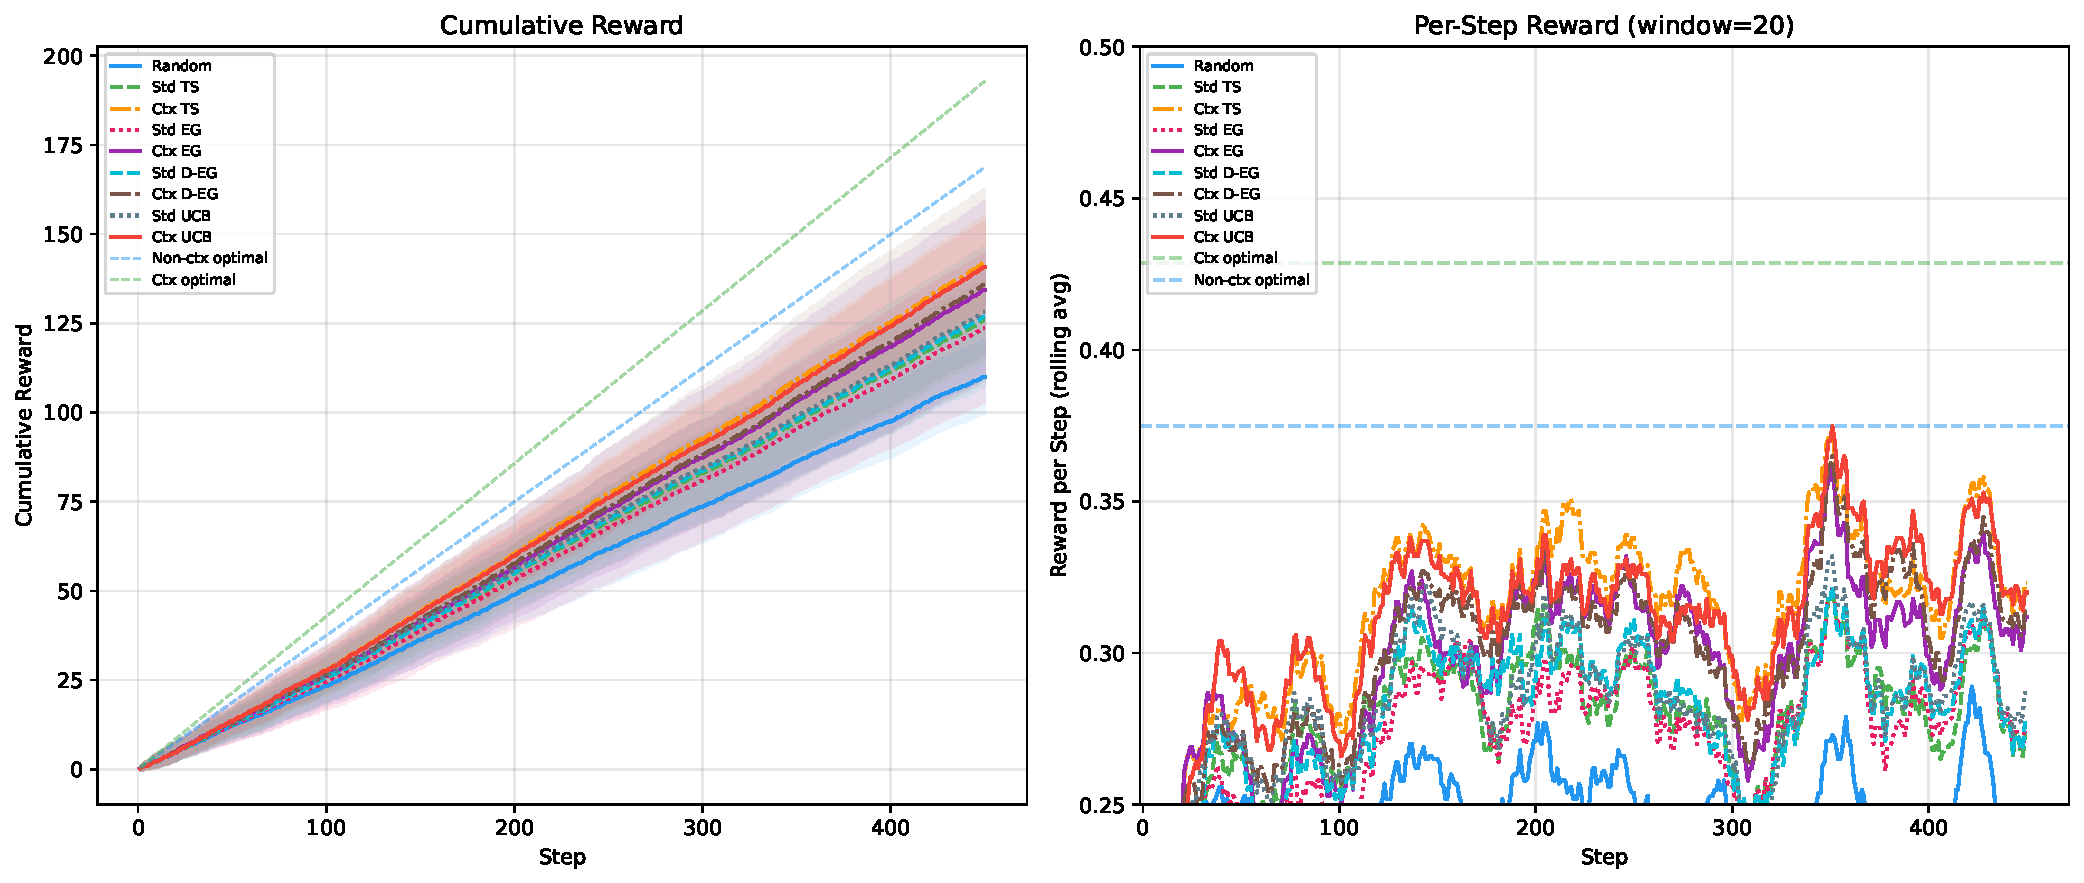
\includegraphics[width=\textwidth]{images/learning_curves_masked.pdf}
\caption{Masked cumulative reward and per-step reward (50 seeds, $\pm$1 SD). Reward floor drops by $20\%$ vs non-masked, but relative ordering is preserved.}
\end{figure}

\section{Known Limitations}

\begin{itemize}
\item Agents are contextual bandits, not state-aware RL. Full state-aware RL (with state history and temporal-difference learning) is Phase 2.
\item Single-timescale reward only. Multi-timescale (immediate + 3-week delayed) is Phase 2.
\item No user response model. Burden accumulation and 4 archetypes are Phase 2.
\item Transition matrix is fixed and known. Learned transitions from real data are Phase 2.
\item Transition probabilities are placeholder values informed by Reactance theory. Calibration against real data is Phase 2.
\end{itemize}

\end{document}
